\begin{figure}[h!]
	\centering
	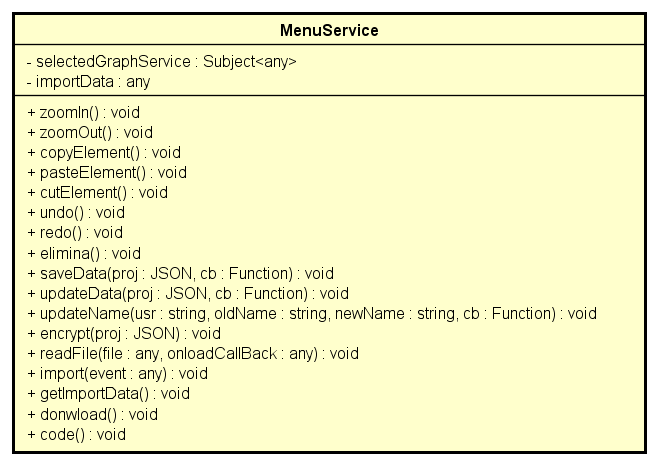
\includegraphics[scale=0.8]{res/sections/SpecificaFrontEnd/Components/Disegnetti/menu.png}
	\caption{Diagramma della classe MenuComponent}
\end{figure}

\begin{itemize}
	\item \textbf{Descrizione:}\\
	È il componente che contiene il \textit{menù}.
	\item \textbf{Utilizzo:}\\
	
	\item \textbf{Attributi:}
		
	\item \textbf{Metodi:}
		\begin{itemize}
			\item \emph{-constructor(private accountService: AccountService)}\\
    		\\
    		\textbf{Parametri:}
    		\begin{itemize}
    		
    			\item \emph{accountService: AccountService}\\
    			
    		\end{itemize}
		\end{itemize}
\end{itemize}